\documentclass{article}
\usepackage{amsmath}
\usepackage{gvv-book}
\usepackage{gvv}
\usepackage{float}
\begin{document}
\begin{enumerate}
	\item The derivative of $\tan^{-1}(x^{2})$ w.r.t. $x$ is:
		\begin{enumerate}
			\item $\frac{x}{1 + x^{4}}$
			\item $\frac{2x}{1 +x^{4}}$
			\item $-\frac{2x}{1 + x^{4}}$
			\item $\frac{1}{1+x^{4}}$
		\end{enumerate}
	\item Overspeeding increases fuel consumption and decreases fuel economy as a result of tyre rolling friction and air resistance. While vehicles reach optimal fuel economy at different speeds, fuel mileage usualy decreases rapidly at speeds above 80km/h. \\
		\begin{figure}[h]
			\centering
			      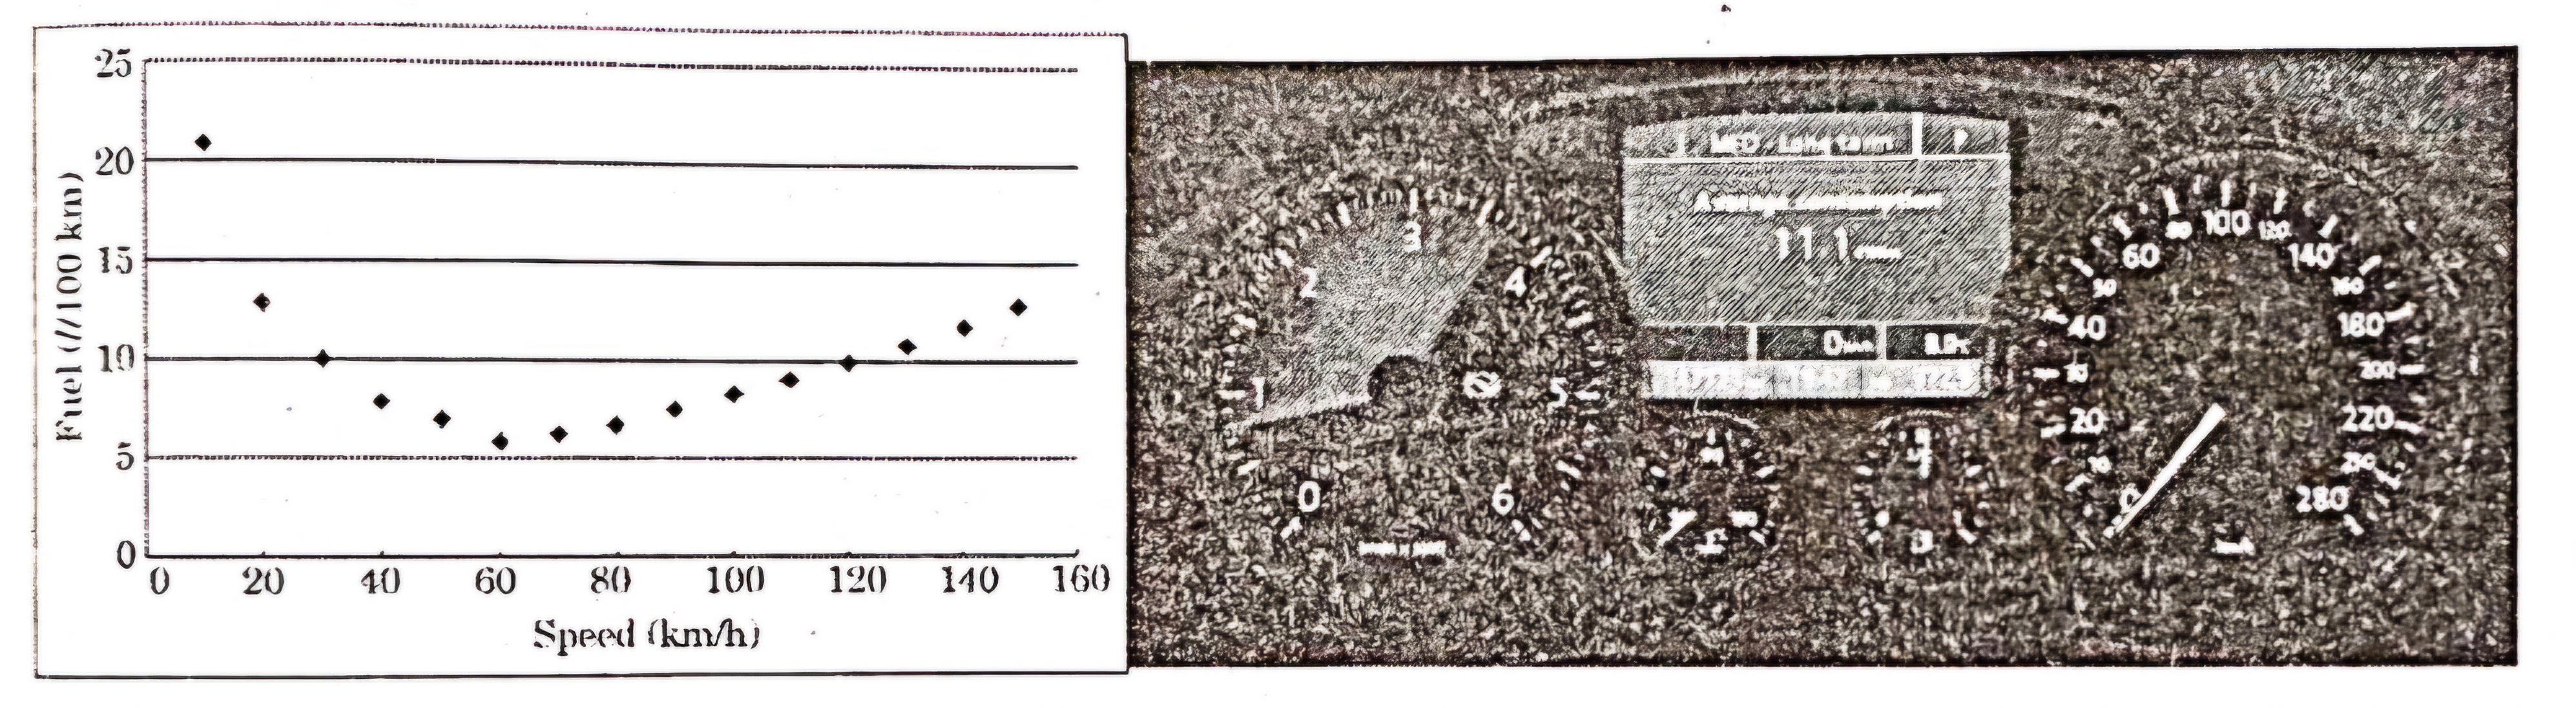
\includegraphics[width=120mm]{./Figuress/Speed.jpg}
			      \caption{1}
			\label{Figure}
		\end{figure}
		The relation btween fuel consumption F(l/100 km) and speed V(km/h) under some constraints is given as $F = \frac{V^{2}}{500} - \frac{V}{4} +14$. \\
		On the basis of the above information, answer the following questions:
		\begin{enumerate}[label=(\roman*)]
			\item  Find F, when $V = 40km/h$.
			\item  Find $\frac{dF}{dV}$.
			\item  Find he speed V for which fuel consumption F is minimum.
			\item  Find the quantity of fuel required to travel 600 km at the speed V at which $\frac{dF}{dV} = -0.01$.
		\end{enumerate}
\end{enumerate}
\end{document}
